
\documentclass[nooutcomes]{ximera}
%\documentclass[space,handout,nooutcomes]{ximera}

% For preamble materials

\usepackage{pgf,tikz}
\usepackage{mathrsfs}
\usetikzlibrary{arrows}
\usepackage{framed}
\usepackage{amsmath}
%\pgfplotsset{compat=1.16}

\graphicspath{
  {./}
  {algorithms/}
  {../algorithms/}
}

\pdfOnly{\renewenvironment{image}[1][]{\begin{center}}{\end{center}}}

%%% This set of code is all of our user defined commands
\newcommand{\bysame}{\mbox{\rule{3em}{.4pt}}\,}
\newcommand{\N}{\mathbb N}
\newcommand{\C}{\mathbb C}
\newcommand{\W}{\mathbb W}
\newcommand{\Z}{\mathbb Z}
\newcommand{\Q}{\mathbb Q}
\newcommand{\R}{\mathbb R}
\newcommand{\A}{\mathbb A}
\newcommand{\D}{\mathcal D}
\newcommand{\F}{\mathcal F}
\newcommand{\ph}{\varphi}
\newcommand{\ep}{\varepsilon}
\newcommand{\aph}{\alpha}
\newcommand{\QM}{\begin{center}{\huge\textbf{?}}\end{center}}

\renewcommand{\le}{\leqslant}
\renewcommand{\ge}{\geqslant}
\renewcommand{\a}{\wedge}
\renewcommand{\v}{\vee}
\renewcommand{\l}{\ell}
\newcommand{\mat}{\mathsf}
\renewcommand{\vec}{\mathbf}
\renewcommand{\subset}{\subseteq}
\renewcommand{\supset}{\supseteq}
\renewcommand{\emptyset}{\varnothing}
\newcommand{\xto}{\xrightarrow}
\renewcommand{\qedsymbol}{$\blacksquare$}
\newcommand{\bibname}{References and Further Reading}
\renewcommand{\bar}{\protect\overline}
\renewcommand{\hat}{\protect\widehat}
\renewcommand{\tilde}{\widetilde}
\newcommand{\tri}{\triangle}
\newcommand{\minipad}{\vspace{1ex}}
\newcommand{\leftexp}[2]{{\vphantom{#2}}^{#1}{#2}}

%% More user defined commands
\renewcommand{\epsilon}{\varepsilon}
\renewcommand{\theta}{\vartheta} %% only for kmath
\renewcommand{\l}{\ell}
\renewcommand{\d}{\, d}
\newcommand{\ddx}{\frac{d}{dx}}
\newcommand{\dydx}{\frac{dy}{dx}}


\usepackage{bigstrut}


\newenvironment{sectionOutcomes}{}{}

\usepackage{array}
%\setlength{\extrarowheight}{-.2cm}   % Commented out by Findell to fix table headings.  Was this for typesetting division?  
\newdimen\digitwidth
\settowidth\digitwidth{9}
\def~{\hspace{\digitwidth}}
\def\divrule#1#2{
\noalign{\moveright#1\digitwidth
\vbox{\hrule width#2\digitwidth}}}


\title{Series}
\author{Bart Snapp and Brad Findell and Jenny Sheldon}
\begin{document}
\begin{abstract}
Problems about series.
\end{abstract}
\maketitle


%\begin{problem}
%Problem
%\begin{freeResponse}
%\begin{hint}
%Hint
%\end{hint}
%\end{freeResponse}
%\end{problem} 

\begin{problem}
A series is the $\answer[format=string]{sum}$ of consecutive terms from a(n) $\answer[format=string]{sequence}$.  

An arithmetic series is the $\answer[format=string]{sum}$ of consecutive terms from a(n) $\answer[format=string]{arithmetic sequence}$.  

A geometric series is the $\answer[format=string]{sum}$ of consecutive terms from a(n) $\answer[format=string]{geometric sequence}$.  
\end{problem}

\begin{problem}
Consider the series: 
\[
1+3+5+7+\dots+99
\]
First compute the sequence of partial sums: 
\[
\begin{array}{c|c} \hline
\text{\# of terms} & \text{Value} \\ \hline
1 & \answer{1} \\
2 & \answer{4} \\
3 & \answer{9}\\
4 & \answer{16}\\
5 & \answer{25}\\
6 & \answer{36}\\
\end{array}
\]
\begin{problem}
Make a conjecture: The sum of the first $n$ terms of this series is $\answer{n^2}$. 

In the series
\[
1+3+5+7+\dots+99
\]
there are $\answer{50}$ terms, so the sum is $\answer{50^2}$.  

\begin{problem}
Noticing patterns is called 
\wordChoice{\choice[correct]{inductive} \choice{productive} \choice{deductive} \choice{reductive}}
reasoning, which is very important in mathematical problem solving. 

But in mathematics, we usually aim to know \textbf{why} patterns works, which requires  
\wordChoice{\choice{inductive} \choice{productive} \choice[correct]{deductive} \choice{reductive}} reasoning.  

Here is picture that can help explain why the sum of the first $n$ odd numbers works out so nicely: 
\begin{image}
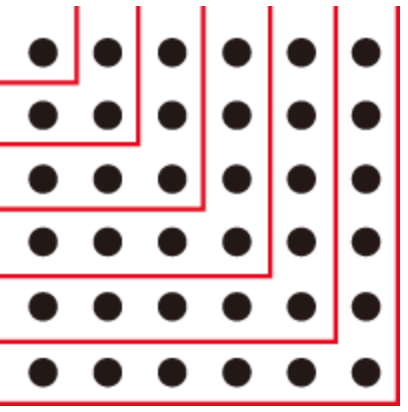
\includegraphics[scale=0.5]{sumOdds.png}
\end{image}

The red lines organize the dots into groups. Moving from the top left toward the bottom right, the number of dots are $\answer{1},\answer{3},\answer{5}$, and so on.  More generally, if $1$ is the first group, then the $n^textrm{th}$ group has $\answer{2n-1}$ dots, which is the $n^textrm{th}$ odd number.  

Furthermore, through the $n^textrm{th}$ odd number, the dots are organized so that they form a square of side length $\answer{n}$, for a total of $\answer{n^2}$ dots.  

This compelling example illustrates an important result:  The sequence of partial sums of a(n) $\answer[format=string]{arithmetic}$ series is a $\answer[format=string]{quadratic}$ function of the number of terms summed.  

The following examples show that patterns are sometimes much harder to see.  
\end{problem}
\end{problem}
\end{problem}


\begin{problem}
Consider the series: 
\[
5+8+11+14+\dots+101
\]
First compute the sequence of partial sums: 
\[
\begin{array}{c|c} \hline
\# of terms & \text{Value} \\ \hline
1 & \answer{5} \\
2 & \answer{5+8} \\
3 & \answer{5+8+11}\\
4 & \answer{5+8+11+14}\\
5 & \answer{5+8+11+14+17}\\
6 & \answer{5+8+11+14+17+20}\\
7 & \answer{5+8+11+14+17+20+23}\\
\end{array}
\]

\begin{problem}
Even suspecting that this sequence is a quadratic function, the pattern is hard to see.  

For arithmetic series, an important and useful technique is as follows. Call the series $S$, and then write out the series forward and backward, with the terms aligned as shown:  
\[
\begin{array}{ccccccccccccccc}
S & = &     5  & + & 8      & + &  11    & + & \cdots & + & 95 & + & 98 & + & 101 \\
S & = & 101 & + & 98 & + & 95 & + & \cdots & + & 11     & + &    8   & + & 5
\end{array}
\]
The terms in each column sum to $\answer{106}$, and there are $\answer{33}$ terms, so on the right, these equations sum to $\answer{106\cdot 33}$.  

But on the left, the equations sum to $\answer{2S}$.  So the sum of the original series is 
$\answer{106\cdot 33/2}$. 

\begin{problem}
Let's generalize this approach to find the sum of the first $n$ terms of the arithmetic series that begins $5+8+11+\dots$.  

First, we need a formula for the $n^{th}$ term in the sequence $5, 8, 11, \dots$.  (Be careful:  It is easy to be ``off by one.'')

If we call 5 the \textbf{first} term, then the $n^{th}$ term is $\answer{5+3(n-1)}$.  
\begin{feedback}
One way of reasoning:  Begin with $5$ and add $(n-1)$ copies of the common difference, which is $3$.  
\end{feedback}

\begin{problem}
For ease of algebra, let's write $5+3(n-1)$ as $3n+2$.  Then proceed as above:  
\[
\begin{array}{ccccccccccccccc}
S & = &     5  & + & 8      & + &  11    & + & \cdots & + & (3n-4) & + & (3n-1) & + & (3n+2) \\
S & = & (3n+2) & + & (3n-1) & + & (3n-4) & + & \cdots & + & 11     & + &    8   & + & 5
\end{array}
\]
The terms in each column sum to $\answer{3n+7}$, and there are $\answer{n}$ terms, so on the right, these equations sum to $\answer{n(3n+7)}$.  

But on the left, the equations sum to $\answer{2S}$.  So the sum of the original series is 
$\answer{n(3n+7)/2}$, which is indeed a $\answer[format=string]{quadratic}$ function of $n$.  
\end{problem}

\end{problem}


\end{problem}


\end{problem}


\end{document}



